\section{Survival of small populations}
\label{m:sec:small}

Return to the binary process of \cref{m:sec:deathordivision} and suppose it is near
critical, either just below or just above. With the probability of division $p$ and
of death $1-p$ each close to a half, a lineage dies at its first round almost half
the time. Should it survive one generation, both its offspring fail at their own
first attempt with probability around $0.25$, so the lineage reaches the second
generation only with probability about $0.375$:
\begin{equation*}
0.375 \approx
\underbrace{(1-0.5)}_{\text{no extinction at the first step}}\times
\underbrace{(1-0.5\times0.5)}_{\text{nor at the second}} .
\end{equation*}

More generally, survival to a given generation is obtained by iterating the \pgf{}.
With $\phi(z)=pz^2+(1-p)$ from \cref{m:eq:pgfbinary}, the extinction and survival
probabilities follow from
\begin{equation}
\label{m:eq:ext}
u_{n+1} = p\,u_n^2 + 1-p,
\qquad
S_{n+1} = 2pS_n - pS_n^2 ,
\end{equation}
started at $u_0=0$, $S_0=1$. At exactly critical branching this gives, for
$n=1,2,3,4$,
\begin{equation*}
u_n = 0.500,\ 0.625,\ 0.695,\ 0.741\qquad(3\ \text{s.f.}),
\end{equation*}
so the probability of survival decays quickly over the first few rounds of
division, and does so almost as fast just above criticality as just below.
\Cref{m:fig:earlySn} makes the point: whatever advantage supercriticality confers, it
is not an early-generation advantage.

\begin{figure}[ht]
\centering
  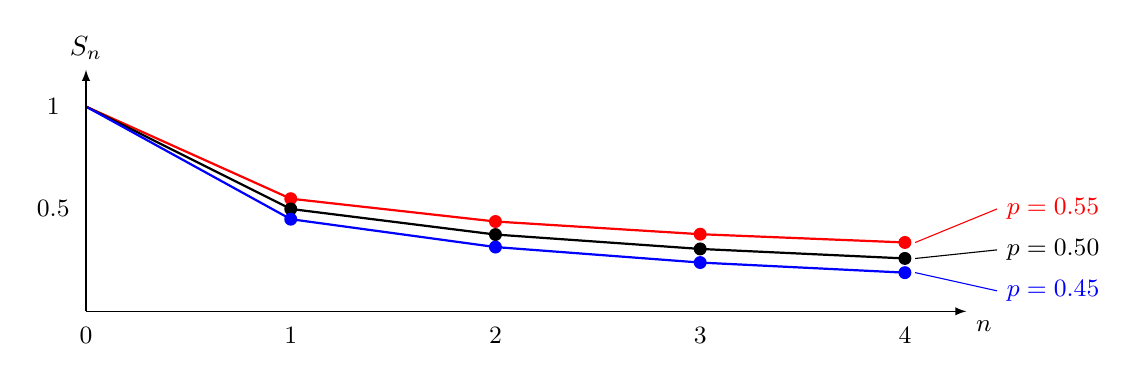
\begin{tikzpicture}[scale = 2.6]
    \foreach \x/\y/\color in {1/0.55/red, 2/0.4386250/red, 3/0.3766719/red, 4/0.336304/red,
                              1/0.5/black, 2/0.375/black, 3/0.3046875/black, 4/0.25827/black,
                              1/0.449999/blue, 2/0.313874/blue, 3/0.2381546/blue, 4/0.188816/blue}
      \fill[color=\color] (\x, \y) circle (0.9pt);
    \draw[red, thick] (0, 1) -- (1, 0.55) -- (2, 0.4386250) -- (3,0.3766719) -- (4,0.336304);
    \draw[black, thick] (0, 1)--(1,0.5) --  (2,0.375) -- (3,0.304687) -- (4,0.25827);
    \draw[blue, thick] (0, 1)--(1,0.449999)  --  (2,0.313874) -- (3,0.238154) -- (4,0.18881);
    \draw[-latex] (0,0) -- (4.3,0) node[below right, font=\small] {$n$};
    \draw[-latex] (0,0) -- (0,1.18) node[above] {$S_n$};
    \foreach \x/\lab in {0/0, 1/1, 2/2, 3/3, 4/4} \node[font=\small] at (\x, -0.12) {\lab};
    \foreach \y/\lab in {0.5/0.5, 1/1} \node[font=\small] at (-0.16, \y) {\lab};
    \draw[red,  thin] (4.05,0.336) -- (4.45,0.50);
    \draw[black,thin] (4.05,0.258) -- (4.45,0.30);
    \draw[blue, thin] (4.05,0.189) -- (4.45,0.10);
    \node[red,  font=\small, anchor=west] at (4.45, 0.50) {$p=0.55$};
    \node[black,font=\small, anchor=west] at (4.45, 0.30) {$p=0.50$};
    \node[blue, font=\small, anchor=west] at (4.45, 0.10) {$p=0.45$};
  \end{tikzpicture}
\caption{Survival probability over the first four generations from a single
progenitor, computed from \cref{m:eq:ext}. Even in the supercritical case
($p=0.55$) the early decay is steep, and the three curves have barely separated by
$n=4$.}
\label{m:fig:earlySn}
\end{figure}

\subsection{An initial cohort of size \texorpdfstring{$k$}{k}}
\label{m:sec:cohort}

Now suppose $Z_0=k$: the process begins not with a single individual but with a
group, small to moderate in number, perhaps $k=10$. Under supercritical branching,
growth becomes more predictably exponential as the count rises, because a large
number of individuals lets the expected dynamics show through the noise of
individual events. The founding cohort is precisely the regime in which that noise
dominates instead.

What, then, are such a cohort's chances of long-run persistence? The question is
answered by asking for the probability that at least one descendant remains, that
is, that not every one of the $k$ founding lineages has died out. The lineages are
independent and each is extinct by generation $n$ with probability $u_n$, so all
$k$ have gone with probability $u_n^{\,k}$, and
\begin{equation}
\label{m:eq:Snk}
S^{(k)}_n = 1-u_n^{\,k} .
\end{equation}
Letting $n\to\infty$ and using \cref{m:sec:certainty}, the ultimate establishment
probability is $0$ for $p\le\tfrac12$ and $1-\bigl((1-p)/p\bigr)^k$ for
$p>\tfrac12$: a larger cohort helps decisively above criticality and not at all
below it, in the long run.

\begin{figure}[ht]
\centering

\includegraphics[width=0.56\textwidth]{kvals.png}
\caption{Survival probability $S^{(k)}_n$ from \cref{m:eq:Snk} out to $500$
generations at exact criticality, $p=0.5$, for $k=1,10,100,1000$ (blue through to
red). A larger founding cohort buys longevity, but at criticality every curve is
still headed for zero.}
\label{m:fig:kvals}
\end{figure}

\begin{figure}[ht]
\centering

\includegraphics[width=0.45\textwidth]{kvals505.png}
\hfill

\includegraphics[width=0.45\textwidth]{kvals495.png}
\caption{As \cref{m:fig:kvals}, but with $p$ displaced slightly from criticality:
$p=0.505$ on the left (supercritical), $p=0.495$ on the right (subcritical). The
benefit of a large initial cohort is acutely sensitive to which side of $\tfrac12$
the process sits on. A displacement of half a per cent separates curves that were
nearly coincident in \cref{m:fig:kvals}.}
\label{m:fig:kvals2}
\end{figure}

\Cref{m:fig:kvals,m:fig:kvals2} show $S_n^{(k)}$ through $500$ generations for
$k=1,10,100,1000$. The effect visible in \cref{m:fig:kvals} --- that a larger first
cohort gives improved longevity --- is highly sensitive to criticality. Persistence
improves quickly as $p$ approaches $\tfrac12$ from below and continues to improve
dramatically into supercriticality, and the two panels of \cref{m:fig:kvals2} differ
only in the third decimal place of $p$.

\subsection{Conditioning and apparent early growth}
\label{m:sec:earlyrep}

The conditioning of \cref{m:sec:qsd} has a mirror image which is worth recording,
because it shows that the effect is not confined to the subcritical case.

Consider an ensemble of independent homogeneous birth--death processes, all with
the same constant rates, and retain only those that happen still to be alive at
some large time. The retained subpopulation is automatically enriched for early
rapid growth: a realisation that grew quickly at the outset is far more likely to
have escaped the early extinction risk documented in \cref{m:fig:earlySn}, and so far
more likely to be in the retained set. No change in the underlying rates is
required to produce the enrichment, and the apparent slowdown that follows is not a
slowdown at all but a reversion to the mean. The effect is known as the \emph{push
of the past}, and was identified in a setting far from the present one, as an
explanation for a systematic pattern in longevity and diversity data
\cite{Budd2018}.

That is exactly the conditioning of \cref{m:sec:qsd} seen from the other side. There
a subcritical process was conditioned on survival and its mean settled to $1/A(p)$
rather than decaying; here a critical or supercritical process is conditioned on
survival to a late time and its early growth appears inflated. In both cases the
conditioning, not the mechanism, does the work. The selection is performed on
trajectories after they have been generated, and the steep early decline of
\cref{m:fig:earlySn} is the source of the resulting bias.

The parallel suggests a modelling hypothesis that later chapters take up: that
early replication weighs heavily on eventual survival, even when later per-capita
rates are unchanged. \Cref{m:fig:earlySn} is the reason to take it seriously, since
the first few generations are where nearly all of the extinction risk sits.

\subsection{Discrete birth--death--catastrophe}
\label{m:sec:bdc}

A birth--death process subject to catastrophe carries, alongside the possibility of
extinction by death, the possibility of an abrupt event that removes the population
at a stroke. In discrete time and up to the point of catastrophe such a process
behaves exactly as the basic Galton--Watson model as far as its limiting
conditional distribution is concerned. Conditioning on non-catastrophe, and
conditioning also on non-extinction by death, it exhibits a stationary limiting
distribution. Whether a quasi-stationary distribution survives when one conditions
on \emph{neither} death nor catastrophe is a separate question, and one best
settled by simulation. Either way it is useful to have the probability of
non-catastrophe in hand.

\subsubsection*{Probability of catastrophe at step \texorpdfstring{$n$}{n}}

Let $\kappa$ be the probability that a given individual initiates catastrophe at a
step. A single individual fails to do so with probability $1-\kappa$, two with
$(1-\kappa)^2$, and a cohort of size $N$ with $(1-\kappa)^N$.

Consider first birth and catastrophe alone, with no death. Then the census of the
living population at any generation is known with certainty: from a single
progenitor the population simply doubles at each step prior to catastrophe. The
process therefore comes to its abrupt halt at generation $n$ with probability
\begin{equation}
\label{m:eq:bdchalt}
1-(1-\kappa)^{2^{\,n-1}},
\end{equation}
one minus the probability that none of the $2^{n-1}$ individuals present caused it.
This is the \emph{conditional} probability of rupture at step $n$ given that every
earlier step was passed, and it should not be confused with the unconditional
probability of the process ending at step $n$.

\subsubsection*{Probability of process survival}

Still with no death, define $S_n$ as the probability that the process survives to
generation $n$. Survival to generation $0$ is certain, $S_0=1$. Survival to
generation $1$ requires only that the founder divided without catastrophe,
$S_1=1-\kappa$. Persistence to step $2$ requires that the founder divided and that
each of its two offspring did too, so $S_2 = (1-\kappa)(1-\kappa)^2$. The pattern
is clear: survival to generation $n$ requires every prior step to have been passed,
and the total exposure over generations $0,\dots,n-1$ is
$1+2+\cdots+2^{n-1} = 2^n-1$, so
\begin{equation}
\label{m:eq:bdcS}
S_n = \prod_{i=0}^{n-1}(1-\kappa)^{2^i}
= (1-\kappa)^{\sum_{i=0}^{n-1}2^i}
= (1-\kappa)^{2^n-1} .
\end{equation}

\subsubsection*{Death included}

The difficulty comes once death is allowed, because the size of the living
population is then no longer known with certainty from one generation to the next.
Let $\widetilde Z_i$ denote the binary Galton--Watson population with the
catastrophe mechanism switched off, and let
\begin{equation}
\label{m:eq:exposure}
H_n = \sum_{i=0}^{n-1}\widetilde Z_i
\end{equation}
be the cumulative exposure over the first $n$ steps. Conditioning on the entire
catastrophe-free genealogy, every individual present independently declines to
trigger, so
\begin{equation}
\label{m:eq:norupture}
\pr{\text{no catastrophe before }n} = \ex{(1-\kappa)^{H_n}} .
\end{equation}
This identity is exact. The natural simplification is to replace the random
exposure by its mean,
\begin{equation}
\label{m:eq:bdcguess}
S_n \overset{?}{=} (1-\kappa)^{\ex{H_n}},
\qquad
\ex{H_n} = \sum_{i=0}^{n-1}(2p)^i
= \begin{cases}\dfrac{1-(2p)^n}{1-2p}, & p\neq\tfrac12,\\[8pt] n, & p=\tfrac12,\end{cases}
\end{equation}
and it is worth being explicit about why this is a heuristic substitution rather
than an identity, because the direction of the error can be pinned down exactly.
The map $h\mapsto(1-\kappa)^h$ is convex, so Jensen's inequality gives
$\ex{(1-\kappa)^{H_n}}\ge(1-\kappa)^{\ex{H_n}}$: replacing the random census by its
mean systematically understates the chance of getting through. Both
\cref{m:eq:bdcguess} and its unconditioned reading are therefore better read as
lower bounds than as equalities. How tight a bound remains a question for numerical
work.

\begin{remark}[A state-dependent catastrophe is not a mean-field hazard]
\label{m:rem:notmeanfield}
The failure of \cref{m:eq:bdcguess} is structural, not a matter of accuracy. Because
the trigger rate depends on the state, the expectation in \cref{m:eq:norupture} is a
nonlinear functional of the whole path, and no substitution of a deterministic
hazard for the random one closes the model. Two further cautions belong with it.
Non-catastrophe is not the same event as population survival: if the requirement is
that the population be both unruptured and non-zero at generation $n$, the exact
probability is
\begin{equation}
\label{m:eq:jointsurvival}
\ex{\ind\{\widetilde Z_n>0\}\,(1-\kappa)^{H_n}},
\end{equation}
for which Jensen's inequality supplies no bound at all, the indicator and the
exposure being negatively associated. And once a trigger occurs every surviving
lineage is stopped together, so the killed lineages are coupled and cannot be
treated as independent after the fact --- although their family trees and trigger
variables do factorise \emph{before} any trigger, which is what makes
\cref{m:eq:norupture} correct and makes the $k$-founder version of it the $k$th
power. Closing the model properly requires a marked or multivariate generating
function, or the killed-generator viewpoint of \cref{m:sec:killedchain}.
\end{remark}

\subsection{Continuous-time birth--death and the constant \texorpdfstring{$\Ac(p)$}{Ac(p)}}
\label{m:sec:cts}

The discrete process resists a closed form for $A(p)$, as \ChA{} shows at length.
Its continuous-time counterpart does not, and it is instructive to see the
continuous calculation carried through completely, because the reason a closed form
exists there is visible at every step, and its absence in discrete time is
correspondingly easier to locate.

Take the linear birth--death process of \cref{m:sec:linbd}, with per-capita birth
rate $\lambda$ and death rate $\mu$, started from $N$ individuals. Its extinction
probability $p_0(t)$ is \cref{m:eq:p0t}, and its survival probability is
$S^{(N)}(t) = 1-p_0(t)$.

\subsubsection*{Limiting mean conditioned on non-extinction}

The process has a stationary conditional mean when $\mu>\lambda$, that is in the
subcritical case. Exactly as in \cref{m:sec:condmean},
\begin{equation}
\label{m:eq:condit}
\ex{X_t\mid X_t>0} = \frac{\ex{X_t}}{S^{(N)}(t)},
\end{equation}
and the late-time limit follows on applying L'Hôpital's rule. It is quicker to take
$N=1$ and compute directly. With $\ex{X_t}=\ee^{(\lambda-\mu)t}$ from
\cref{m:eq:bdmean} and, from \cref{m:eq:p0t},
\begin{equation}
\label{m:eq:ctsS}
S(t) = 1-\frac{\mu-\mu\ee^{(\mu-\lambda)t}}{\lambda-\mu\ee^{(\mu-\lambda)t}}
= \frac{\lambda-\mu}{\lambda-\mu\ee^{(\mu-\lambda)t}},
\end{equation}
\cref{m:eq:condit} gives
\begin{equation}
\label{m:eq:ctscondmean}
\ex{X_t\mid X_t>0}
= \frac{\ee^{(\lambda-\mu)t}\lrb{\lambda-\mu\ee^{(\mu-\lambda)t}}}{\lambda-\mu}
= \frac{\lambda\ee^{(\lambda-\mu)t}-\mu}{\lambda-\mu} .
\end{equation}
This is the whole calculation, and the point to notice is what it did \emph{not}
require. The survival probability \cref{m:eq:ctsS} is available in closed form for
every $t$, not merely asymptotically, because the generating function
\cref{m:eq:bdsolution} solves the birth--death equation exactly; the amplitude of
its exponential decay can therefore be read straight off. Rearranging
\cref{m:eq:ctsS} as
\begin{equation*}
S(t) = \frac{\mu-\lambda}{\mu}\,\ee^{-(\mu-\lambda)t}
\lrb{1-\frac{\lambda}{\mu}\ee^{-(\mu-\lambda)t}}^{-1}
\;\sim\;\frac{\mu-\lambda}{\mu}\,\ee^{-(\mu-\lambda)t}
\qquad(t\to\infty),
\end{equation*}
the continuous-time analogue of the amplitude $A(p)$ is exhibited outright: it is
the prefactor $(\mu-\lambda)/\mu$. Nothing here is a limit of accumulated
early-time corrections; the early behaviour is contained in the same elementary
expression as the late behaviour.

For $\mu>\lambda$ the exponential in \cref{m:eq:ctscondmean} decays, and the limiting
conditional mean is the constant
\begin{equation}
\label{m:eq:ctsqsmean}
\lim_{t\to\infty}\ex{X_t\mid X_t>0} = \frac{\mu}{\mu-\lambda}
= \frac{1}{1-\lambda/\mu}
\;\lrb{=\frac{1}{\Ac}} ,
\end{equation}
the reciprocal of the prefactor just identified, exactly as $1/A(p)$ is the
reciprocal of the discrete amplitude in \cref{m:eq:qsmean}.

\subsubsection*{Matching the two parametrisations}

To compare this with the discrete-time constant the two parametrisations must be
matched, and \cref{m:prop:race} is what matches them: with birth and death clocks
running at rates $\lambda$ and $\mu$, the probability that the birth clock wins is
\begin{equation}
\label{m:eq:pfromrates}
p = \frac{\lambda}{\lambda+\mu},
\qquad\text{so that}\qquad
\frac{\lambda}{\mu} = \frac{p}{1-p} .
\end{equation}
The embedded jump chain of the birth--death process is then precisely the
discrete-generation model with division probability $p$. In that parametrisation
\begin{equation}
\label{m:eq:Acts}
\frac{1}{\Ac} = \frac{1-p}{1-2p},
\qquad\text{that is}\qquad
\Ac(p) = \frac{1-2p}{1-p} = \frac{2\varepsilon}{1+\varepsilon},
\end{equation}
with $\varepsilon=1-2p$ as in \cref{m:eq:epsdef}, the subscript marking this as the
continuous-time constant, to distinguish it from the discrete-time $A(p)$ of
\cref{m:eq:lateS}. Its properties are elementary and complete: $\Ac$ is a rational
function of $p$, decreasing from $\Ac(0)=1$ to $\Ac(\tfrac12^-)=0$, and near
criticality $\Ac(p)\to2\varepsilon$.

\subsubsection*{Discrete against continuous}

Set the two constants side by side:
\begin{equation}
\label{m:eq:twoconstants}
\Ac(p) = \frac{1-2p}{1-p}\quad\text{(closed form)},
\qquad
A(p) = \lim_{n\to\infty}\frac{S_n}{(2p)^n}\quad\text{(a limit, and no more)} .
\end{equation}
\Cref{m:fig:dtct} plots them together and raises the obvious question: why does the
continuous curve start at $1$ where the discrete one starts at $\tfrac12$, given
that the two agree at the critical end? A factor of two at one endpoint and none at
the other means that no constant rescaling of $\Ac$ can reproduce $A$.

The reason a closed form was available for $\Ac$ and is not available for $A$ can
be stated precisely. In continuous time the survival probability solves a linear
first-order equation whose solution \cref{m:eq:ctsS} is elementary at every $t$; the
amplitude is a value of that solution. In discrete time the survival probability
obeys the quadratic recursion \cref{m:eq:SnIter}, whose late behaviour is geometric
but whose amplitude is the accumulated product of every early nonlinear correction,
as \cref{m:sec:riccati} showed the continuum approximation cannot supply. Discreteness
of the generational clock is exactly what obstructs the closed form.

The comparison is taken up properly in \ChA, which proves the strict bound
$A(p)>\tfrac12\Ac(p)$, shows that the ratio $A/\Ac$ increases monotonically from
$\tfrac12$ at $p=0$ to $1$ at $p=\tfrac12^-$, accounts for both endpoints, and
explains the obstruction structurally. For present purposes it is enough to record
that $A(p)$ exists, that $\Ac(p)$ is its elementary continuous-time analogue, that
the two are of the same order near criticality, and that $A(p)$ must be computed
rather than evaluated.

\begin{figure}[ht]
\centering

\includegraphics[width=0.5\textwidth]{dtctA.png}
\caption{The continuous-time constant $\Ac(p) = (1-2p)/(1-p)$ (green) against
high-precision numerical values of the discrete-time constant $A(p)$ (red points).
Both vanish at $p=\tfrac12$, but at $p=0$ the continuous curve starts at $1$ and
the discrete one at $\tfrac12$, and the two are not related by a constant factor in
between. The black line is a formula obtained by symbolic regression; it tracks the
points closely but is not exact, and \ChA{} both accounts for the discrepancy
between the two curves exactly and explains why the fitted curve cannot be right.}
\label{m:fig:dtct}
\end{figure}

\subsection{Continuous-time birth--death--catastrophe}
\label{m:sec:ctbdc}

The discrete process of \cref{m:sec:bdc} has a continuous-time counterpart, and since
it is the central object of several later chapters it is defined here, in the
notation established above. No results about it are derived in this chapter.

\begin{definition}[Birth--death--catastrophe process]
\label{m:def:bdc}
Let $X_t$ count individuals in a compartment. Each individual independently gives
birth at rate $\lambda$ and dies at rate $\mu$, and the compartment additionally
undergoes a catastrophe --- a rupture that removes the entire population at once
--- at a rate $\rho$ per individual, so that the total catastrophe rate in state
$n$ is $\rho n$. Writing $\dagger$ for the post-catastrophe state, the non-zero
transition rates out of $n\ge1$ are
\begin{equation}
\label{m:eq:bdcrates}
q_{n,n+1} = \lambda n,
\qquad
q_{n,n-1} = \mu n,
\qquad
q_{n,\dagger} = \rho n ,
\end{equation}
and both $n=0$ and $\dagger$ are absorbing.
\end{definition}

Two features distinguish \cref{m:def:bdc} from the linear birth--death process of
\cref{m:sec:linbd}, and both matter later. The process now has \emph{two} absorbing
states, reached by mechanisms that are distinguishable and not interchangeable:
extinction empties the compartment gradually, catastrophe empties it in one event
and releases its contents. And the catastrophe rate is proportional to the
population, so the compartment becomes more likely to rupture the fuller it is.

The generating-function machinery of \cref{m:sec:pgf} applies unchanged. Restricting
attention to realisations that have not yet ruptured and writing
$G(z,t) = \ex{z^{X_t}\ind\{X_t\neq\dagger\}}$, the master equation for
\cref{m:eq:bdcrates} yields
\begin{equation}
\label{m:eq:bdcpde}
\pddt{G} = \bigl(\lambda z^2-(\lambda+\mu+\rho)z+\mu\bigr)\pdd{G}{z},
\qquad G(z,0) = z^{N},
\end{equation}
which differs from \cref{m:eq:bdpde} only in the coefficient of $z$. The quadratic no
longer factorises with a root at $z=1$, and that single change is responsible for
most of what is interesting about the process: probability is not conserved on the
non-ruptured states, and $G(1,t)$ is the survival probability rather than one.
Rates, means and variances, state probabilities and the associated
generating-function equations are developed \fwd{bdc}{in the later chapters on
birth--death--catastrophe processes}, with the two-type extension treated
\fwd{multitype}{in the chapter on multi-type processes} and the release of a
ruptured compartment's contents into a shared medium
\fwd{rupture}{in the chapter on compartment rupture}. The method used to solve
\cref{m:eq:bdcpde} and its relatives is the subject of \cref{m:sec:moc}.

\subsection{Catastrophe as a killed chain}
\label{m:sec:killedchain}

The birth--death--catastrophe models can be placed in a common framework without
introducing their full parameter catalogues, and the framework is worth having here
because it is what connects catastrophe to the conditioning of \cref{m:sec:qsd}. Let
the positive state $i$ carry birth rate $\lambda_i$, ordinary death rate $\mu_i$
and catastrophe rate $\kappa_i$, a catastrophe sending the process directly to $0$:
\begin{equation}
\label{m:eq:bdcgeneralrates}
i\longrightarrow i+1 \ \text{at rate }\lambda_i,
\qquad
i\longrightarrow i-1 \ \text{at rate }\mu_i,
\qquad
i\longrightarrow 0 \ \text{at rate }\kappa_i .
\end{equation}
The jump $1\to0$ may therefore occur by either mechanism. On bounded test functions
the generator is
\begin{equation}
\label{m:eq:bdcgenerator}
(\mathcal Lf)(i)
= \lambda_i\{f(i+1)-f(i)\} + \mu_i\{f(i-1)-f(i)\} + \kappa_i\{f(0)-f(i)\},
\qquad i\ge1,
\end{equation}
with $(\mathcal Lf)(0)=0$. Linear birth and death correspond to
$\lambda_i = i\lambda$ and $\mu_i = i\mu$, and \cref{m:def:bdc} to
$\kappa_i = i\rho$; the catastrophe sequence may remain general.

Restricting the generator to the positive states gives the \emph{killed}
subgenerator $K$, with off-diagonal entries $K_{i,i+1}=\lambda_i$ and
$K_{i,i-1}=\mu_i$ for $i\ge2$, and diagonal
\begin{equation}
\label{m:eq:killedsubgen}
K_{i,i} = -(\lambda_i+\mu_i+\kappa_i) .
\end{equation}
The row mass missing from $K$ is exactly the instantaneous absorption rate: it is
$\kappa_i$ for $i\ge2$, and $\mu_1+\kappa_1$ for $i=1$. Writing
$T_0 = \inf\{t\ge0 : X_t = 0\}$ and summing the positive-state forward equations,
\begin{equation}
\label{m:eq:bdcsurvivalloss}
\ddt{}\pr{T_0>t}
= -\mu_1\pr{X_t=1} - \sum_{i\ge1}\kappa_i\pr{X_t=i},
\end{equation}
all probabilities on the right being understood before absorption. Ordinary death
removes survival mass only from state $1$; catastrophe can remove it from every
positive state, and that asymmetry is the whole difference between the two channels.

The same balance sharpens the connection with quasi-stationarity. If a distribution
$\nu = (\nu_i)_{i\ge1}$ on the positive states is quasi-stationary in the sense of
\cref{m:def:qsd} and the relevant sums are finite, then for some $\theta>0$
\begin{equation}
\label{m:eq:bdcqsdeigen}
\nu K = -\theta\nu,
\qquad
\mathbb{P}_\nu\!\left(T_0>t\right) = \ee^{-\theta t} .
\end{equation}
Indeed quasi-stationarity writes the unnormalised positive-state law at time $t$ as
$a(t)\nu$; the semigroup property forces $a(s+t) = a(s)a(t)$, and right-continuity
gives $a(t)=\ee^{-\theta t}$. Differentiating at zero yields the left eigenvector
relation, and summing its coordinates against \cref{m:eq:bdcsurvivalloss} identifies
the decay rate,
\begin{equation}
\label{m:eq:bdcdecayrate}
\theta = \mu_1\nu_1 + \sum_{i\ge1}\kappa_i\nu_i .
\end{equation}
A quasi-stationary law is thus a left eigenvector of the killed generator, and its
eigenvalue is the survival decay rate --- the continuous-time statement of what
$A(p)$ and $(2p)^n$ do together in \cref{m:eq:lateS}.

One limiting case is worth isolating. If $\kappa_i\equiv\kappa$ is constant on the
positive states, the catastrophe clock may be taken independent of the underlying
birth--death process, and the killed semigroup factorises,
\begin{equation}
\label{m:eq:constantcatastrophe}
P^K_t = \ee^{-\kappa t}P^{\mathrm{BD},K}_t .
\end{equation}
The extra clock shifts the survival decay rate by $\kappa$ and leaves the law
conditional on survival unchanged. A state-dependent sequence such as
$\kappa_i = i\kappa$ behaves quite differently: it weights paths by their
accumulated population exposure --- the quantity $H_n$ of \cref{m:eq:exposure} in
its continuous-time form --- and generally changes the quasi-stationary law itself.
That distinction, and the eigenrelation \cref{m:eq:bdcqsdeigen}, are all the present
chapter needs; the later chapters build on both.

\FloatBarrier
